\documentclass[10pt,titlepage]{article}
\usepackage[utf8]{inputenc}
\usepackage[margin=1in]{geometry}
\usepackage{amsmath}
\usepackage{amsfonts}
\usepackage{amssymb}
\usepackage{indentfirst}
\usepackage{graphicx}
\usepackage[section]{placeins}
\usepackage{listings}

\setlength{\parindent}{24pt}

\title{Monte Carlo simulation for background studies in NPOL at C-GEN}
\date{\today}
\author{William Tireman\\ Department of Physics, Northern Michigan University \and Daniel Wilbern, Northern Michigan University}

\begin{document}
\maketitle

\section{Introduction}
We have developed a Monte Carlo simulation for the purpose of simulating the effects of background radiation on the neutron-proton recoil polarimeter for the E12-11-009 (C-GEN) collaboration at Jefferson National Laboratory Hall C.  This simulation was written in C++ and uses the Geant4 particle physics simulation toolkit and the ROOT data analysis framework.

This document details how to setup and use the simulation, how to modify the simulation's geometry, and how the simulation's output data is stored for use in analysis scripts.

\section{Quick Setup}

\subsection{Building nmu-npol}

nmu-npol requires Geant4 and ROOT to be installed and their environments properly initialized by their respective shell scripts.  CMake is required in addition to build nmu-npol.

The source files for nmu-npol are available on Github.  To get and build the simulation for the first time:
\begin{lstlisting}[frame=single]
git clone https://github.com/JeffersonLab/nmu-npol
cd nmu-npol
./cleanBuild
cd build
\end{lstlisting}

The cleanBuild script runs CMake, compiles the simulation and analysis program, and places build files including the executable in the appropriate build directory.  The simulation is placed in ``build/simulation'' while the analysis program is placed in ``build/analysis''. Once the program has been build for the first time, future rebuilds can be performed by changing directory to the appropriate build directory and then running 'make'.  If new classes are added to the code then cleanBuild will have to be run again.

\subsection{Running nmu-npol}
\subsubsection{Running in Interactive Mode}
Once nmu-npol is compiled, its execution is controlled by macro files.  The simulation can be run in visualization mode or batch mode.  To run in visualization mode, simply run the Npolapp executable with no arguments:
\begin{lstlisting}[frame=single]
cd /path/to/nmu-npol/build/simulation
./Npolapp
\end{lstlisting}
This runs the init-vis.mac (or init.mac if Geant4 was not built with support for visualizations) macro file and brings up the Geant4 Qt user interface. \\

\subsubsection{Running with Macro Files}
The nmu-npol version since July 2016 now uses the generalized particle source class.This class gives the user more control over the generated particles in the macro file.  This includes the ability to bias particle distributions for energy(momentum), xyz initial position, and initial momentum direction via theta and phi distributions. All macro files contain three common commands which can be changed to adjust the primary particle's type, how often the simulation outputs its progress, and how many total events should be simulated.  In the electron beam macro file, these values are:
\begin{lstlisting}[frame=single]
/gun/particle e-
/run/printProgress 10000
/run/beamOn 10000000
\end{lstlisting}

The new generalized particle generator has spawned two main macro files and can support an number of others based on user needs.  The first file is called ElectronBeam.mac and produces a beam of electrons in a circular 2-mm wide pattern pointed in the +z-direction. The user can change the initial position, beam energy, beam profile, direction, and several other parameters from this file as they see fit. \\

The second macro file is a particle generator designed to produce particles on a flat source and bias the particle generations for initial energy, position (x,y), and momentum direction (theta, phi angles).  The idea is to reproduce the particle distributions from the analysis of the particle flux through two tagger volumes in the full electron beam on target simulation.  This will allow for targeted analysis of the setup without the need to run the much longer runs of electrons on target over and over again. \\

The name of the macro file is ParticleFlux.mac.  There are two 'tagger' volumes for which biasing histogram for energy, xy, theta, and phi have been analyzed for 9 particle species.  The data files are stored in' build/simulation/macros/particleFluxData'.  The two taggers are descried below. There is a special requirement that must be done before running the biased macro.  These changes are to the simulation setup and require the code to be recompiled.  First, in NpolDetectorConstruction.cc file you must comment out all unnecessary elements such as beam line, all shell, scattering chamber. If generating particles at the NPOL tagger then comment out the shield hut and dipole magnets as well.  Then you will need to go into NpolPolarimeter.cc, NpolParticleFluxTagger.cc, and NpolShieldHut.cc and change the variable at the top called "NpolAng" from 28.0 degrees to 0.0 degrees.  This is necessary in order to get the theta biasing correct. \\

	This macro was developed to bias the event generator with distributions of particles at a "tagger" volume. The tagger volumes are placed in the full simulation with electron beam on target to track particles initially crossing those volumes as a way to determine the flux of various particles through those surfaces. The tagger volumes are as follows. \\  
	
	The "Target tagger" is a thin volume placed very close to the entrance of Dipole 1 (Charybdis). The idea is to capture flux data from electron scattering in the target, scattering chamber, beam line elements, etc. for future analysis. \\

	The "Npol tagger" is a thin volume placed very close to the front wall of the polarimeter shield hut on the inside of the shield hut.  This tracks particles that manage to get through both magnets, the collimator, and the lead curtain. \\

	The "SHMS tagger" is a thin volume placed very close to the horizontal bender magnet's entrance. \\

	To run with the biased particle flux, the user has to comment/uncomment the appropriate lines in the macro file.  They also have to choose the correct particle flux data files on the lines loading in the histogram points.  For example, if you wish to generate particles at the NPOL tagger, then uncomment all lines for NPOL tagger source setup and the /control/execute "filename" lines which reference the NPOL tagger.  Then make sure the files being loaded are for the particle you are studying.  For example, if you want to look at neutrons on the polarimeter you would make sure all files loading have the word "neutron" in the name. Also make sure you have set the primary particle to neutron as well at the top of the macro. \\

\subsubsection{Output files from batch mode}
When nmu-npol is run in batch mode, the output directory, output filename prefix, number of events saved per file, and job number may be specified by the NPOLDIR, NPOLBASENAME, NPOLEVENTSPERFILE, and JOBNUMBER environment variables.  If these environment variables are not set, the default output directory is ./output, the default output filename prefix is npol, the default number of events per file is 100,000 and the default job number is 99999.  To set these variables and execute Npolapp in batch mode:
\begin{lstlisting}[frame=single]
cd /path/to/nmu-npol/build/simulation
export NPOLDIR=/path/to/output_dir
export NPOLBASENAME=npol\_basename
export NPOLEVENTSPERFILE=100000
export JOBNUMBER=1
./Npolapp npol.mac
\end{lstlisting}
Using the default values will result in the ROOT output file(s) being saved to the ./output directory with name(s) npol\_99999\_XXXXX.root where XXXXX is the five digit file number starting with 00001. If you use the above ENV settings, the name will be npol\_basename\_1\_00001.root for the first file and increment the file number for each new file.  \\

\subsubsection{Running Multiple Jobs on a Local Machine}
The NMUsetuprun.sh and NMUjobsubmit.sh scripts can be used to easily run several batch jobs at once.  Edit the NMUsetuprun.sh file with the correct location of the nmu-npol build dir and the desired environment variables, then run NMUjobsubmit.sh with the number of desired jobs as an argument.  The jobs will be run in the background.  For example, on a quad core machine you may wish to run four jobs at once:
\begin{lstlisting}[frame=single]
cd /path/to/nmu-npol/build/simulation
emacs scripts/NMUsetuprun.sh # set environment variables
source scripts/NMUsetuprun.sh
./scripts/NMUjobsubmit.sh 4
\end{lstlisting}
The script may also be run with two arguments: the starting job number of the batch and the number of jobs to run.  If you already have output files from four jobs in the output directory, you may want to run e.g. \texttt{./scripts/NMUjobsubmit.sh 5 4} instead.

\subsection{Running on the JLab Farm}
Currently, running on the JLAB batch farm is an exercise in patience (Summer 2016). In order to attempt to incorporate multithreading, it was necessary to move to ROOT version 6.x.  This invokes needed to use C++11 standards which invokes needing a new OS kernel (linux version 3.x or higher ... if memory serves). The good folks at JLAB, including efforts by Bob Michaels to compile ROOT 6.x, has resulted in the necessary parts being in place.  Referencing them when submitting a job to the batch farm is another chore which I will state my success here. \\

Insert section about ENV for running Npolapp \\

Once you are on the JLAB farm, you can run the same as you would do on your local machine in interactive mode.
\begin{lstlisting}[frame=single]
cd /path/to/nmu-npol/build/simulation
./Npolapp
\end{lstlisting}
Just remember to setup as described above on the Jlab farm interactive system before attempting to compile and run.  Remember to run only tests on the JLAB interactive farm.  Play nice in the sandbox. \\

If you wish to run on the batch farm nodes, then a job submission script needs to create a jobsub file and then submit the job with the jsub command. You may need to modify the job submission script (JLABjobscript.csh) to generate jobsub files with the correct information (user name, job name, etc.). Then modify the JLABsetuprun.csh script which sets directories and environmental variables as necessary. Then to submit a number of jobs to the farm nodes do the following:
\begin{lstlisting}[frame=single]
  cd build/simulation/scripts	# do this after you have completed a build
  ./JLABjobscript.csh i j
\end{lstlisting}
This script will generate the jobsub file, submit the job, pause for 1 seconds (take a breath), and then generate the next one and submit until all have been submitted between i and j where i is the first job number and j is the last job number with i $<$ j.  Note that these job numbers are used in the ROOT file identification so you MUST watch your file names and job numbers. You could overwrite previous runs. User beware! \\
	 
In the job submission script is an ENV variable called 'NPOLEVENTSPERFILE'. This variable sets the number of events allowed to be generated by the primary generated before a ROOT file is closed out and a new one is opened as dicussed in section 2.2.3.  It is recommended to run with about 100k events per file and then combine the files together later using the ROOT command 'hadd'.  For a 10 million event run, there would be 100 files for the entire run.  If 1000 jobs are submitted then a total of 100,000 files would be generated.  If the groups of 100 files will add up to be less than about 10-20 GB then it is beneficial to combine them together using the ROOT command 'hadd'. This can be done by using the following.
\begin{lstlisting}[frame=single]
  cd location_of_files
  hadd -k -f npol_basename_jobnumber.root npol_basename_jobnumber_*.root
\end{lstlisting}
The options -k and -f allow for bad ROOT files to be skipped and not to crash the command. The first file string is the output ROOT file and the second file string contains the wildcard character '*'.  A more sophisticated shell script could be written to perform this operation and then delete the files once the operation has completed successfully to save space on the drives.  If not then the user must clean up the space manually.  The user could also write into the shell script a command to submit the file to the tape silos for long term storage. \\

\section{Simulation Geometry}

\begin{figure}[ht]
  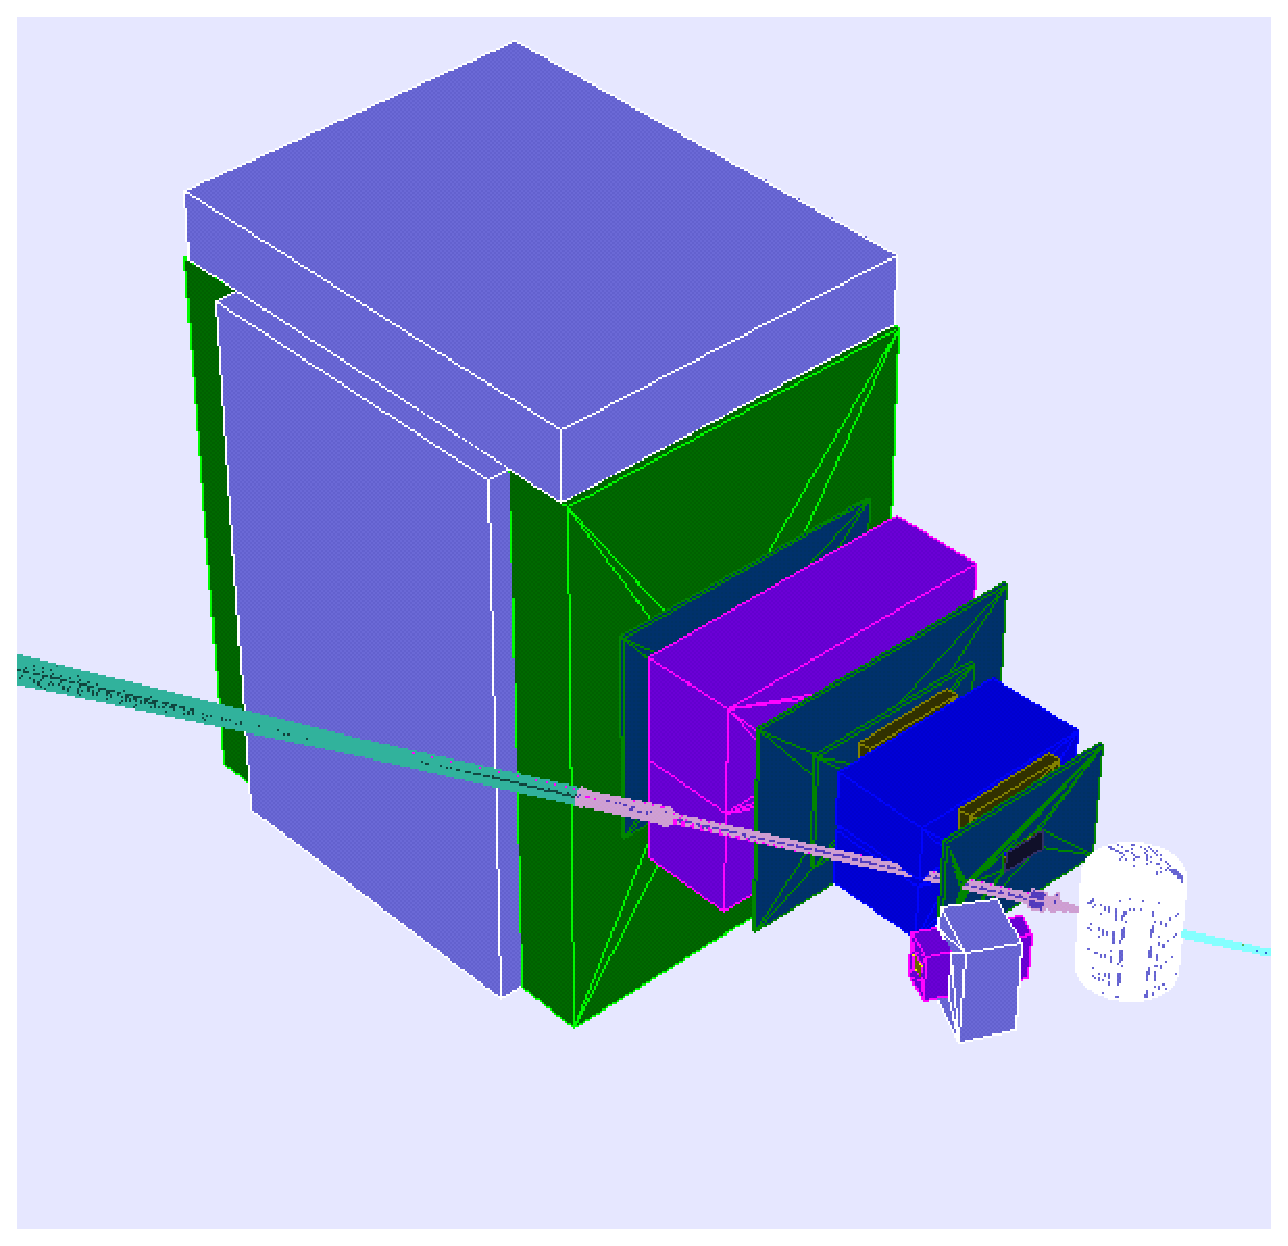
\includegraphics[scale=0.5]{figures/geometry}
\caption{Simulated Hall C geometry.}
\label{fig:geometry}
\end{figure}

Figure \ref{fig:geometry} shows the current implementation of the simulated Hall C geometry for C-GEN.  In this geometry, the following objects are implemented: the scattering chamber with LD2 target inside, upstream and downstream beam-lines, SHMS H-bender magnet, two dipole magnets, and shield hut with the NPOL neutron-proton recoil polarimeter inside.

\subsection{Materials}

The NpolMaterials singleton class handles the materials definitions of the nmu-npol simulation, which allows for many volumes in the simulation to use the same common materials without redefining them. Custom materials are stored in an STL map keyed by the name of the material as a string.  To add a custom material to the singleton, create a new method that returns the material as a G4Material *.  Then add a line to \texttt{NpolMaterials::CreateMaterials()} that adds the material to the map of custom materials.

To access materials defined in NpolMaterials, call \texttt{NpolMaterials::GetMaterial(const G4String material)} with the material's name as the argument.  For example, to get the custom-defined material named "Concrete":
\begin{lstlisting}
G4Material *concrete = NpolMaterials::GetInstance()->GetMaterial("Concrete");
\end{lstlisting}
This method first searches the map of custom-defined materials, then G4NistManager, then G4Material.  If no material by that name is found, NULL is returned.  

\subsection{Simulation Geometry}

Geant4 allows one to construct and place objects in the simulated environment if its attributes (shape, material, location, etc.) are specified.  The nmu-npol simulation uses the abstract factory pattern of object-oriented design to implement the simulated experiment hall.  This design allows for a modular implementation of the simulation's geometry. 

Each object in the hall is constructed and placed by a factory class that inherits from NpolDetectorFactory.  To build an object in the simulated hall geometry, define a class that is a subclass of NpolDetectorFactory, implement the construction of solids and logical volumes in the constructor, and implement the abstract virtual methods \texttt{Place(G4LogicalVolume *motherLV)} and \texttt{GetName()}.  The Place method should create a G4VPhysicalVolume inside the provided mother volume.  NpolDetectorFactory provides the PlaceRectangular and PlaceCylindrical methods, which allow for the simple placement of a logical volume by specifying rectangular or cylindrical polar coordinates in the mother volume's coordinate system.

The NpolDetectorConstruction functions as a builder and places each specified volume inside the world volume.  To have an object placed directly in the world, add it to the list of constructed objects in NpolDetectorConstruction's constructor.  When placing objects in the world, the coordinate system is defined such that the LD2 target is at the origin and the downstream beam-line runs along the positive z-axis.

\subsection{Magnetic Fields}

The magnetic fields in the two dipole magnets for the NPOL side were implemented using the G4Uni-formMagField class.  The SHMS horizontal bender magnet currently does not have a magnetic field implemented since it is far enough from the beamline to not effect the electron beam and any secondary particle generation would be generally away from the NPOL shield hut entrance. A TOSCA map for the horizontal magnet exists at Hall C in the case that studies around the SHMS are necessary. \\

The magnets for NPOL are labeled dipole 1 and dipole 2 in the code and have the common names Charybdis and BNL48D48 respectively. In Geant 4.10 and higher, the sensitive detectors and magnetic fields must be assigned in detector construction.  There is also a requirement that the magnetic field be assigned to a specific logical volume.  In order to accomplish this in the individual constructors, a base method in NpolDetectorConstruction is used to assign volume to the detector map which is really a map of all volumes in the world. In the individual constructors, a method which constructs the magnetic field and assigns it to the logical volume is implemented. \\

The specifics of the magnetic fields for dipoles 1 and 2 are as follows. A volume made of ``soft vacuum'' is placed in the opening of each magnet. The volume is then assigned a uniform magnetic field generated by G4UniformMagField and points in the positive y-direction.  The transport manager is set to 1.0-mm maximum step length and the field is interpolated using the G4ClassicalRK4 class.  The minimum step is set to 0.0025-mm. \\

Lastly, the strength of the dipole field can be adjusted at the top of each dipole constructor.  The current setup splits the integrated field equally between the two magnets. The user can perform any combination they want.  Currently there is no implementation to use a TOSCA map for the two dipoles. \\

\section{Simulation Output and Analysis}

The nmu-npol simulation uses the NpolAnalysisManager and NpolFileManager singleton classes to handle data from the simulation, organize it into data structures, and have it written to output files.  Analysis of these data files is done by ROOT scripts separate from the simulation itself.

The output file contains two TTrees: one that is filled at the end of each simulated event and one that is filled just before the file is closed.  The ``T" TTree stores information at the per-event level.  This tree has branches containing data about the events' vertecies, simulation steps, and particle flux tagger volume hits.  Each entry in this TTree is data about one event.

The ``T2" TTree has just one branch with a single entry containing an STL vector with a single element: an NpolStatistics object that contains some information about the file.   This object contains the number of simulated events that were written to the file, the total number of events simulated including ones that were not written to the file, and a version number that is updated whenever there is a major change to the output file structure.  Not every simulated event is stored in ``T", so this information may be necessary in analysis scripts to calculate statistical quantities like cross-sections or particle fluxes that depend on the number of electrons on target.

\subsection{Output Files}

The simulation output files are in the ROOT file format.  These files are written to the location specified by the NPOLDIR enviornmental variable and have their filename prefixed with the NPOLBASENAME and JOBNUMBER enviornment variables.  If these variables are not specified, the default is to write them to output/npol\_99999\_\#.root.  The simulation outputs several files in sequence; a file is closed and a new one is opened every time the number of events specified in the enviornment variable NPOLEVENTSPERFILE (or 100,000 events by default) are simulated.  Each time a new file is opened, its suffixed file number is incremented.  The totalEvents member of each file's NpolStatistics object should be equal to the number provided in NPOLEVENTSPERFILE except perhaps for the last file of the run if the total number of events simulated is not an exact multiple of NPOLEVENTSPERFILE.  To output a single file for the entire run of the simulation, NPOLEVENETSPERFILE can be set to 0, but we reccomend outputting many files and processing them in ROOT analysis scripts using a TChain.

\subsection{Simulation Stepping Data, Particle Flux Taggers, and Event Selection}

Each entry of the ``steps" branch of the ``T" TTree in the output files is an STL vector containing NpolStep objects.  Each NpolStep object stores some information about a simulation step: the time the step occured, the energy deposited during that step, and the name of the volume the step occured in.  The NpolStep objects in the STL vector are sorted in time order, allowing analysis routines to iterate through the vector, sum energy deposition in desired volumes, and record the time when this energy deposition meets a certain threshold.

To facilitate measurement particle flux rates at certain locations in the simulation's geometry, ``tagger" volumes are placed in important locations and data about steps that occur in these volumes is saved to the output file.  There are currently three tagger volumes in the simulation: NpolTagger behind the collimator in the polarimeter shield hut, SHMSTagger in front of the SHMS horizontal bending magnet, and ParticleTagger in front of the dipole magnet closest to the target.  For each tagger volume, there is a branch in the ``T" TTree containing an STL vector of NpolTagger objects, which each contain data about a step that occurred inside the tagger volume.

To cut down on the size of the output files, which are already typically quite large, we do not store data about all events in the output files.  Currently we store data about events with at least one step in the ParticleTagger volume in front of the dipole magnet closer to the target.

\subsection{Simulation Tracking Data}

The ``tracks" branch contains data about the tracking vertices of the simulation in an STL vector containing NpolVertex objects.  Each NpolVertex object contains data about a tracked particle in the simulation when it was created.  These NpolVertex objects are stored in the vector at index determined by the track ID, so beware that some entries in the vector may be NULL if there was no track ID with that index.

\end{document}

